\documentclass[../main.tex]{subfiles}

\begin{document}
\section{Densities from Densities}


While bar graphs and histograms can give asense of the variability in
data, they are limited to showing the dispersion of the data only in how the measurements are spread out. This is somewhat limiting for very large datasets, so the boxplot has evolved as a way to display more characteristics of the distribution \cite{wickham2011}. While a simple boxplot does not inherently show conditional dependencies, many derviations do. 


\begin{figure}
  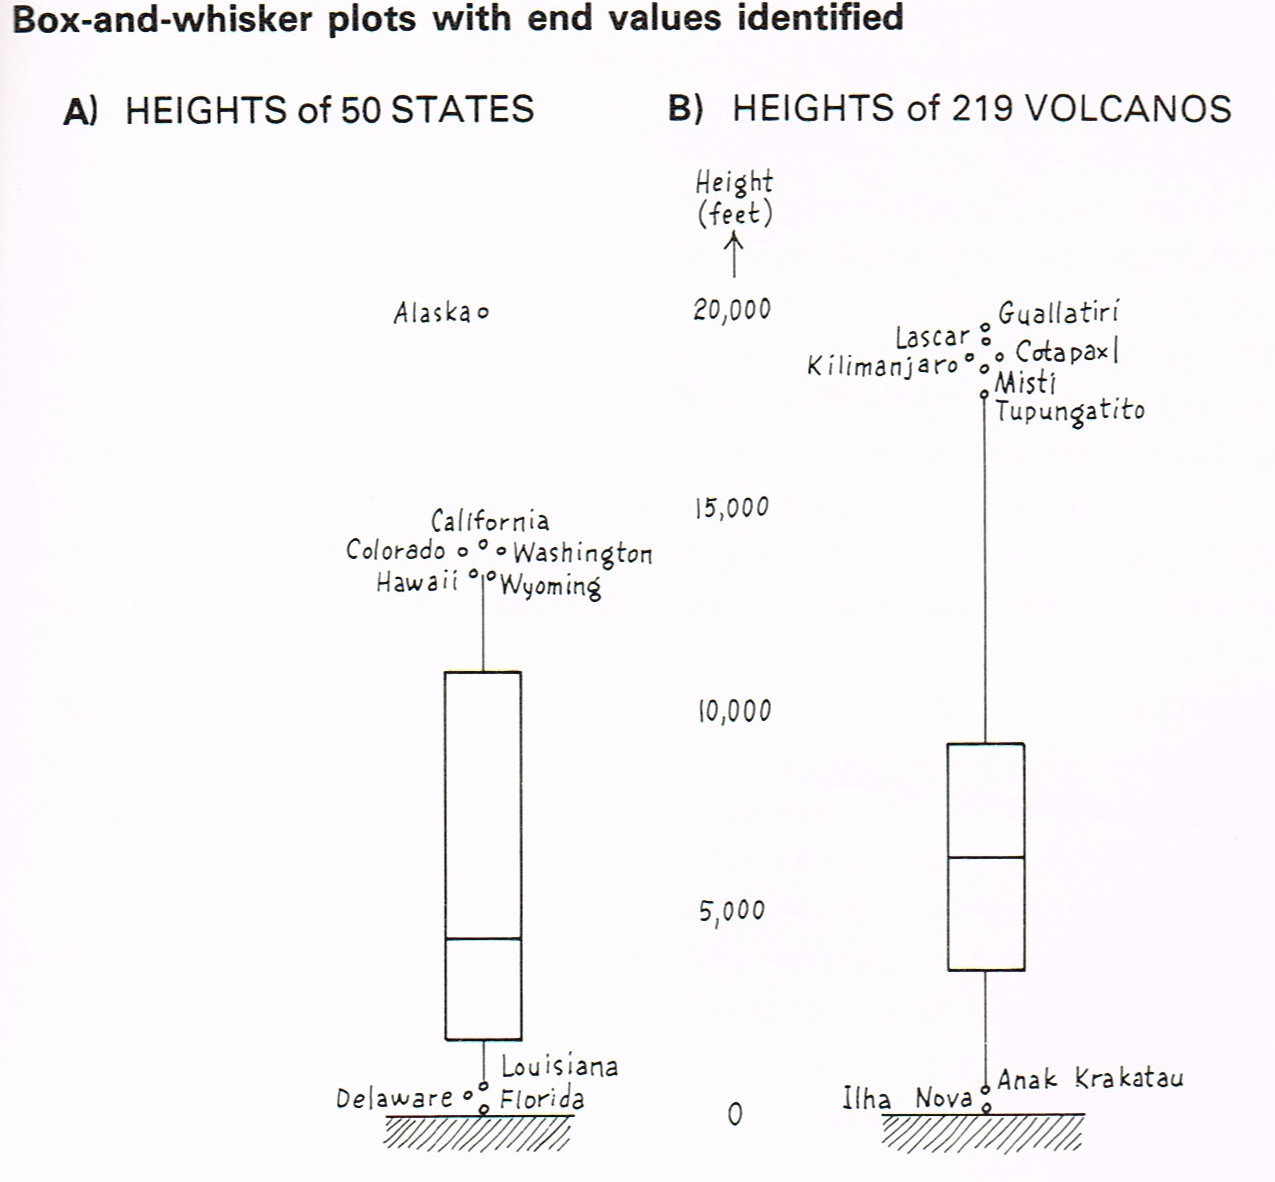
\includegraphics{boxplot}
  \caption{Tukey's 1977 example of the box plot (exhibit 6 of chapter 2 from
    Exploratory Data Analytics\cite{tukey1977}) illustrates how the box plot
    shows
    the distribution of topology of states and
    the distribution of volcanos. The strength of the box and whisker is that
    the
    reader can quickly compare the two distributions and learn, for example,
    that
    volcanos tend to span a shorter range of average heights, but that the
    extremes
    are much further from the center. Essentially, the distributions act as
    references for the other displayed distributions.}
  \label{fig:boxplot}
\end{figure}

Tukey's introduction to the boxplot \cite{tukey1977}, shown in
Figure~\ref{fig:boxplot} illustrates how the distributions of these 1d densities differ by category. While this graph shows the median, range between upper and lower interquartile, and lower and upper extreme, many authors have exploited the structure to convey more information about the data. Authors used different quantile levels \cite{hyndman1996}s or measures of outliers
\cite{frigge1989}, or ways of identifying outliers\cite{carter2009,
  schwertman2004, schwertman\
  2007}, or otherwise incorporated skewness,
kurtosis, and other descriptive distributional statistics \cite{kim2004,
  hubert2008, marmolejo\
  2015}.








